\documentclass[a4paper,11pt,titlepage,french]{article}
% classe de document pour LaTeX qui définit les paramètres généraux du document : 
    % a4paper : définit le format de papier sur lequel le document doit être imprimé (a4paper format standard)
    % 11pt : définit la taille de police de base à 11 points
    % titlepage : demande à LaTeX d'insérer une page de titre dans le document
    % french : Cette option indique à LaTeX que le document est rédigé en français
% TODO : \input{chemin vers le fichier de setup} 
    % le fichier de setup devra contenir l'ensemble des usepackage suivants et les variables globales
% ----------------
% LIBRAIRIES LATEX
% ----------------
\usepackage[main=french]{babel}
\usepackage[T1]{fontenc}
\usepackage{fontspec}
\usepackage{fancyhdr}
\usepackage{xspace, graphicx}
\usepackage{longtable}
\usepackage[table]{xcolor}
\usepackage{hyperref}
\usepackage{enumitem}	
\usepackage{listings}
\usepackage{tcolorbox}
\usepackage{color}
\usepackage{courier}

% To use animUML example.tex file
\usepackage[T1]{fontenc}
\usepackage{graphicx}
\usepackage[export]{adjustbox}
\usepackage{float}

\usepackage{caption}
\usepackage{lastpage}

% ------------------
% VARIABLES GLOBALES
% ------------------
\newcommand{\version}{1.0}
\newcommand{\revision}{0}
\newcommand{\documentName}{Manuel d'installation}
\newcommand{\documentNameAbrev}{INST}
\newcommand{\prose}{ProSE}
\newcommand{\creator}{Elisa DECLERCK}
\newcommand{\projectName}{Passerelle Android-CAN vers banc CAN réel ou simulé} % TODO
\newcommand{\annee}{2024}
\newcommand{\teamName}{CANvengers} 
\newcommand{\teamNumber}{B1}
\newcommand{\client}{KEREVAL}
\newcommand{\nomLogiciel}{CANgateway} 
\newcommand{\nomApplication}{CANdroid} 

\setcounter{secnumdepth}{4} % Pour avoir une numérotation jusqu'au niveau 4
\renewcommand{\theparagraph}{\thesubsubsection.\arabic{paragraph}} % Pour numéroter les paragraphes à partir du niveau 3
\makeatletter % Redéfinit la commande \paragraph pour qu'elle utilise les paramètres de formatage de la commande \subsubsection.
\renewcommand\paragraph{\@startsection{paragraph}{4}{\z@}%
    {-3.25ex \@plus -1ex \@minus -.2ex}%
    {1.5ex \@plus .2ex}%
    {\normalfont\normalsize\bfseries}}
\makeatother
\setlength{\parindent}{0pt} % Supprime l'indentation par défaut

% -------------------------------------------------------
% --------------------------
% PARAMETRES HEADER / FOOTER 
% --------------------------
\pagestyle{fancy} % permet de personnaliser l'apparence de l'en-tête et du pied de page de chaque page du document
\setlength{\hoffset}{-40pt} % définis la marge horizontale gauche
\setlength{\topmargin}{-25pt} % définis la marge supérieure 
\setlength{\headsep}{10pt} % définis l'espace vertical entre l'en-tête et le corps de texte 
\renewcommand{\headheight}{60pt} % redéfinis la hauteur de l'en-tête
\renewcommand{\headwidth}{450pt} %  redéfinis la largeur de l'en-tête
\setlength{\textwidth}{450pt} % définis la largeur du corps de texte
\setlength{\textheight}{604pt} %  définis la hauteur du corps de texte
\renewcommand{\footrulewidth}{0.1mm} % redéfinis la largeur de la ligne de séparation de pied de page
\fancyhf{} % vide les entêtes et pieds de page précédemment définis
    % HEADER %
    \fancyhead[LO]{\bf \includegraphics[width=80pt]{../figures/eseo.png}\\ % fancyhead - personnaliser l'en-tête avec 2 arguments : orientation "LO" pour "Left Odd" / contenu "\bf" pour texte en gras + "\includegraphics" inclure le logo de l'ESEO
        \medskip % ajoute espace vertical moyen (≃ 6 points)
        {\prose} équipe {\teamNumber} {\annee}} % texte en dessous de l'image de la partie gauche du pdf
    \fancyhead[RO]{\bf 
\includegraphics[width=90pt]{../figures/logo_kereval.png}\\ % fancyhead - personnaliser l'en-tête avec 2 arguments : orientation "RO" pour "Right Odd" / contenu "\bf" pour texte en gras + "\includegraphics" inclure le logo de l'entreprise
        {\small{Ref. {\documentNameAbrev}\_{\teamNumber}}}} % texte en dessous de l'image de la partie droite du pdf
    % FOOTER %
    \fancyfoot[LO]{\sl {\it Version {\version} - Révision {\revision}}} % fancyfoot - personnaliser le pied de page avec 2 arguments : position "LO" pour "Left Odd" / contenu "\sl" + "\it" pour texte en italique de la version et la révision
    \cfoot{\copyright {\annee} Droits réservés {\teamName}} % insérer texte au centre du pied de page
    \fancyfoot[RO]{\thepage/\pageref{LastPage}} % pied de page partie droite : numéro de page
% ------------------------------
% FIN PARAMETRES HEADER / FOOTER 
% ------------------------------
\definecolor{darkWhite}{rgb}{0.90,0.90,0.90}

\lstset{
    backgroundcolor=\color{darkWhite},
    breakatwhitespace=false,
    breaklines=true,
    commentstyle=\color{red},
    deletekeywords={...},
    escapeinside={\%*}{*)},
    keywordstyle=\color{blue},
    language=bash,
    stepnumber=0,
    stringstyle=\color{orange},
    tabsize=4,
    columns=fullflexible, 
    title=\lstname,
}

\lstdefinestyle{frameStyle}{
    basicstyle=\footnotesize,
    numbers=left,
    numberstyle=\tiny\color{black}
}
 
\tcbuselibrary{listings,skins,breakable}
 
\newtcblisting{customFrame}{
    width=\textwidth,
    listing only,
    listing options={style=frameStyle}
}

% --------------
% DEBUT DOCUMENT 
% --------------
\begin{document}
\sloppy % relâche les règles de justification de texte pour éviter des espaces trop larges
\renewcommand{\arraystretch}{1.3} % augmente la hauteur des lignes d'un tableau

%-----------------------------------------------
%   The titles of the parts
%-----------------------------------------------
\makeatletter
% Adds a sub-subparagraph level
\newcounter{subsubparagraph}[subparagraph]
\renewcommand\thesubsubparagraph{%
    \thesubparagraph.\@arabic\c@subsubparagraph}
\newcommand\subsubparagraph{%
    \@startsection{subsubparagraph}               % counter
    {6}                                           % level
    {0em}                                         % indentation
    {1em}                                         % before the title
    {1em}                                         % after the title
    {\normalsize\hspace{6em}\color{colorTitle}} % style (overloaded by the title format)
}
\newcommand\l@subsubparagraph{\@dottedtocline{6}{13em}{6em}}
\newcommand{\subsubparagraphmark}[1]{}
\providecommand*{\toclevel@subsubparagraph}{6}

\setcounter{tocdepth}{6}    % Allows the paragraph in the table of contents
\setcounter{secnumdepth}{6} % Allows the numbering of the sub-paragraph

\makeatother
% -------------------
% PAGE DE GARDE {p.1}
% -------------------
\begin{center} % centre le contenu de la commande
    \vspace*{2cm} % ajout d'espace
    \rule[0.5ex]{0.7\textwidth}{0.1mm}\\ % ajout ligne horizontale : décalage verticale "ex" / largeur de page "%" / épaisseur "mm"
    \vspace*{2mm} % ajout d'espace
        {\Huge {\textsc{\bf {\documentName}}}} % crée un titre : police en gras "\bf" / petites capitales "\textsc" / grande taille polile "\Huge" 
    \vspace{0.4cm}\\ % ajout d'espace / "\\" : retour à la ligne 
        {\large\bf {\prose} {\teamNumber} {\annee} - {\teamName}}\\ % crée un titre : police en gras "\bf" / taille de police relativement grande "\large"
    \vspace*{1mm}
        {\large\bf {\projectName}}\\ % crée un titre 
    \rule[0.5ex]{0.75\textwidth}{0.1mm}\\ % ajout ligne horizontale
    \vspace{2cm} 
    \begin{tabular}{|c|c|} % crée un tableau avec 2 colonnes 
        \hline % crée une ligne dans le tableau // & : séparateur colonne
            Responsable du document & {\creator}                      \\
            État du document        & En réalisation                  \\
            Version                 & {\version}                      \\
            Révision                & {\revision}                     \\
        \hline
    \end{tabular}
\end{center}
\vspace{3cm} 
% -------------------
% AVERTISSEMENT {p.1}
% -------------------
\noindent % supprime l'indentation automatique au début d'un paragraphe
\textbf{AVERTISSEMENT :} % titre avertissement en gras
\vspace{3mm} \\
Le présent document est un document à but pédagogique.  
Le document de conception ci-joint est strictement confidentiel et réservé à un usage interne. 
Il a été réalisé sous la direction de Jérôme DELATOUR, en collaboration avec des enseignants 
et des étudiants de l'option SE du groupe ESEO. Ce document est la propriété de Jérôme DELATOUR, du groupe ESEO.
Toute utilisation, diffusion ou reproduction de ce document sans autorisation écrite préalable de Jérôme DELATOUR est interdite. 
Nous tenons à souligner que toute violation de cette politique pourrait engager la responsabilité civile et pénale de son auteur. 
Nous vous demandons de prendre toutes les précautions nécessaires pour assurer la sécurité et la confidentialité de ce document.
% -----------------------
% FIN PAGE DE GARDE {p.1}
% -----------------------
 
% ---------------------
% TABLEAU VERSION {p.2}
% ---------------------
% \noindent % Modifie l'espacement horizontal entre les colonnes
%
% Tableau des version à remplir à chaque fois que vous apportez une modification
%
\newpage % nouvelle page 
\begin{center}
\begin{longtable}[l]{|p{2cm}|p{5.8cm}|p{2.8cm}|p{1.4cm}|p{1.7cm}|}
    \hline
        \textbf{Date} & \textbf{Actions} & \textbf{Auteur} & \textbf{Version} & \textbf{Révision}\\
    \hline
        05/04/2023 & Création du document & Elisa\newline Declerck & 0.0 & 0\\
    \hline
        03/04/2023 & Réalisation du diagramme de séquence de "Démarrer le SàE" & Paul\newline  TRÉMOUREUX & 0.0 & 1 \\
    \hline
        07/04/2023 & Rédaction de Portée & Gabriel\newline MARQUETTE & 0.0 & 2\\
    \hline
        07/04/2023 & Rédaction de Objet & Gabriel\newline  MARQUETTE	& 0.0 & 3 \\
    \hline
        08/04/2023 & Réalisation de certains diagrammes de séquence & Théo\newline  BÉNARD & 0.0 & 4 \\	
    \hline
        10/04/2023 & Correction des diagrammes de séquence & Elisa\newline  DECLERCK & 0.0 & 5 \\	
    \hline
        12/04/2023 & Rédaction de la machine à états de Sender & Gabriel\newline  MARQUETTE & 0.0 & 6\\
    \hline
        12/04/2023 & Rédaction des descriptions des classes Sender, Basket et Network & Gabriel\newline  MARQUETTE & 0.0 & 7\\
    \hline
        12/04/2023 & Rédaction de la description générale des classes suivante : GUI, UI, Dealer, Logger, Object, Frame, Sniffer & Paul\newline  TRÉMOUREUX & 0.0 & 8\\
    \hline
        12/04/2023 & Rédaction de diagrammes de séquence & Thomas\newline  ROCHER & 0.0 & 9\\
    \hline
        12/04/2023 & Rédaction de diagrammes de séquence & Camille\newline  LENNE & 0.0 & 10\\
    \hline
        13/04/2023 & Correction du CU "Démarrer le SàE" & Paul\newline  TRÉMOUREUX & 0.0 & 11\\
    \hline
        13/04/2023 & Relecture et correction des doublons de descriptions générales de toutes les classes & Paul\newline  TRÉMOUREUX & 0.1 & 0\\
    \hline
        13/04/2023 & Rédaction de la description de l'architecture candidate & Elisa\newline  DECLERCK & 0.1 & 1\\
    \hline
	    13/04/2023 & Ajout des multiplicitées au diagramme de classe & Elisa\newline  DECLERCK & 0.1 & 2\\
    \hline
        15/04/2023 & Relecture des parties Références, Types de données et Services Offerts & Camille\newline LENNE & 0.1 & 3 \\
    \hline
        15/04/2023 & Relecture et correction de la description des diagrammes de séquence & Camille \newline LENNE & 0.1 & 4\\
    \hline
        16/04/2023 & Correction CU Reconnecter l'application {\nomApplication} & Thomas\newline  ROCHER & 0.1 & 5\\
    \hline
        16/04/2023 & Correction de la description de l'architecture candidate & Thomas\newline  ROCHER & 0.1 & 6\\
    \hline
        16/04/2023 & Inclusion de la MAE de GUI	& Elisa\newline  DECLERCK & 0.1 & 7 \\
    \hline
        17/04/2023 & Relecture section 2.2 + rédaction de note & Thomas\newline  ROCHER & 0.2 & 0\\		
    \hline
        17/04/2023 & Relecture partie + rédaction de note & Gabriel\newline  MARQUETTE & 0.2 & 1\\
    \hline
        17/04/2023 & Rédaction de la description de la MAE & Elisa\newline  DECLERCK & 0.2 & 2\\
    \hline
        18/04/2023 & Correction du schéma et de la description de la MAE de GUI & Elisa\newline  DECLERCK & 0.2 & 3\\
    \hline
        18/04/2023 & Correction de la section 2.2 & Thomas\newline  ROCHER & 0.2 & 4\\
    \hline
        19/04/2023 & Correction du dossier dans sa globalité & Théo\newline  BÉNARD & 1.0 & 0\\
    \hline
        26/04/2023 & Correction de certaines descriptions des diagrammes de séquence & Elisa\newline  DECLERCK & 1.0 & 1\\
    \hline
        27/04/2023 & Création de la MAE de UI et rédaction de sa description & Elisa\newline  DECLERCK & 1.0 & 2\\
    \hline
        27/04/2023 & Correction de la MAE de GUI & Gabriel\newline  MARQUETTE & 1.0 & 3\\
    \hline
        27/04/2023 & Correction de l'ensemble du dossier à la suite de l'audit consultatif & Elisa\newline  DECLERCK & 1.0 & 3\\
    \hline
        30/04/2023 & Relecture de la partie CANgateway de la conception détaillée & Thomas\newline  ROCHER & 1.1 & 0\\
    \hline
        24/05/2023 & Ajout de l'architecture du programme {\nomLogiciel} & Elisa\newline  DECLERCK & 1.1 & 1\\
    \hline
        26/05/2023 & Correction de la MAE de GUI & Elisa \newline DECLERCK & 1.1 & 2\\
    \hline
        26/05/2023 & Rédaction de la description des classes du programme {\nomLogiciel} & Elisa \newline DECLERCK & 1.1 & 3\\
    \hline
        28/05/2023 & Rédaction de la description des classes proxyGUI, proxyLogger, Dispatcher et Postman du programme {\nomLogiciel} & Thomas \newline ROCHER & 1.1 & 4\\
    \hline
        30/05/2023 & Rédaction des différents diagrammes de classes & Gabriel \newline MARQUETTE & 1.1 & 5 \\    
    \hline
        30/05/2023 & Rédaction du protocole de communication & Thomas \newline ROCHER & 1.1 & 6 \\    
    \hline
        31/05/2023 & Relecture de la conception détaillée & Thomas \newline ROCHER & 1.2 & 0 \\    
    \hline
        05/06/2023 & Correction dossier de conception & Elisa \newline DECLERCK & 1.2 & 1 \\
    \hline
        05/06/2023 & Correction et relecture de la conception détaillée coté Android & Camille \newline LENNE & 1.2 & 2 \\
    \hline
        09/06/2023 & Correction du dossier après audit normatif de code & Elisa \newline DECLERCK & 1.2 & 3 \\
    \hline
        13/06/2023 & Correction du dossier de conception dans sa globalité & Thomas \newline ROCHER & 2.0 & 0 \\
    \hline

\end{longtable}

\captionof{table}{Table des évolutions et validations internes du document}
\end{center}
\newpage % nouvelle page 
% -------------------------
% FIN TABLEAU VERSION {p.2}
% -------------------------

\newpage
% --------------
% SOMMAIRE {p.3}
% --------------
\tableofcontents % génére table des matières en fonction des commandes "\section{}"
% ------------------
% FIN SOMMAIRE {p.3}
% ------------------
\newpage

% ------------
% INTRODUCTION
% ------------
% Auteurs : Camille Constant, Paul Trémoureux

\section{Introduction}
\label{sec:intro}

\subsection{Contexte}
\label{sec:intro:contexte}

\noindent\begin{tabularx}{\linewidth}{|p{3.5cm}|X|}
\hline
{\bf Produit à tester :} & {\projet} - version {\versionProjet}\\
\hline
{\bf Type de produit :} & {\produit}.\\
\hline
{\bf Commanditaire :} & {\client}\\
\hline
{\bf Développeur :} & {\equipe}\\
\hline
{\bf Testeur :} & {\equipe}\\
\hline
\end{tabularx}

\subsection{Objet}
\label{sec:intro:objet}

Ce document décrit l'activité de test système qui sera menée par {\equipe} durant le projet {\projet} dans le but de valider le produit suivant : {\produit}. Il est rédigé sous la responsabilité du Responsable Qualité-Test (RQT), sous la direction du Chef de Projet (CdP), conformément au Plan d'Assurance Qualité Logicielle (PAQL) élaboré sous la responsabilité du RQT (cf. section~\ref{sec:eqTest}, Équipe de test).

\subsection{Portée} 
\label{sec:intro:portee}

Sont concernés par ce document :
\begin{itemize}
    \item les testeurs : afin que ceux-ci connaissent le périmètre des tests (ce qu'ils vont tester), l'environnement de test (comment les tests seront mis en {\oe}uvre) et le processus de test (comment s'y prendre et rendre compte des résultats lors de l'exécution des tests) ;
    \item les développeurs : à titre informatif, afin que ceux-ci sachent comment va être validée leur production ; à titre indicatif afin qu'ils sachent, par la description de la gestion des anomalies, comment ils s'interfaceront avec l'équipe de test ;
    \item le client : ce plan de test fait l'objet d'une contractualisation avec le client pour déterminer le périmètre des tests menés pour valider le produit livré et les niveaux d'acceptation de cette validation ;
    \item les auditeurs : ce plan de test, ainsi que son implication, feront l'objet d'audits par la société Formato.
\end{itemize}

\subsection{Copyright}
\label{sec:intro:copyright}
Cf. {\refPAQL} (section 1.3. Copyright).

\subsection{Présentation du système} 
\label{sec:intro:scope}

Le système développé est un ensemble de 2 programmes : une application Android nommé {\appliA} déployé sur un smartphone Android et un programme C nommé {\appliC} déployé sur une Raspberry Pi.
L'application {\appliA} sera relié au programme {\appliC} par un réseau TCP/IP. La Raspberry Pi sera connectée à un réseau CAN pour dialoguer avec Tableau de Bord (soit banc de test physique soit simulateur sur un PC).
Ce projet permettra d'envoyer des trames depuis l'application {\appliA} vers Tableau de Bord afin de piloter ce dernier à distance.

\subsection{Références}
\label{sec:intro:ref}

\subsubsection{Documents de référence internes}
\noindent\begin{tabularx}{\linewidth}{|p{3cm}|X|p{1.4cm}|X|}
\hline
\textbf{Ref.} & \textbf{Nom et auteur} & \textbf{Version} & \textbf{Source}\\
\hline
{\refSpec} & Dossier de spécifications - \newline {\equipe} & 2.0.0 & se2024-b1.doc/specification/livrables\\
\hline
%Si client impliqué dans le PAQL
{\refPAQL} & Plan d'Assurance Qualité Logiciel - {\rqt} & 1.0.0 & pdf sur le dépôt\\
\hline
\end{tabularx}

\subsubsection{Documents de référence externes}
\noindent\begin{tabularx}{\linewidth}{|p{2.8cm}|X|}
\hline
\textbf{Ref.} & \textbf{Nom} \\
\hline
[ISO-829-2008] & Documentation de test logiciel\\
\hline
[ISO/IEC/IEEE 29119-1:2022] & Ingénierie du logiciel et des systèmes - Essais du logiciel - Partie 1: Concepts généraux\\
\hline
\end{tabularx}

\subsection{Glossaire et abréviations}
\label{sec:intro:termes}

Ce sont les termes et abréviations nécessaires à la compréhension de l'activité de test (les termes techniques propres au projet seront indiqués dans le dossier de spécification).

\subsubsection{Abréviations}

\noindent\begin{longtable}[c]{|p{.20\textwidth}|p{.80\textwidth}|}
\hline
CdP & Chef de Projet\\
\hline
IHM & Interface Homme-Machine\\
\hline
PAQL & Plan Assurance Qualité Logicielle\\
\hline
RQT & Responsable Qualité et Test\\
\hline
\end{longtable}

\subsubsection{Glossaire}

\noindent\begin{longtable}[c]{|p{.20\textwidth}|p{.80\textwidth}|}
\hline
{\bf Campagne de test} & Activité qui consiste à dérouler un ensemble de jeux de test. Un dossier de test est produit à l'issue d'une campagne.\\
\hline
{\bf Cas de test} & Déclinaison d'un test précisant les valeurs utilisées pour les variables du test ainsi que les résultats attendus.\\
\hline
{\bf Dossier de test} & Ensemble documentaire qui contient la description des scénarios et des cas de tests, ainsi que l'exécution des jeux de test. Le dossier de test est le reflet d'une campagne de test. \\
\hline
{\bf Jeux de test} & Ensemble des scénarios et cas de tests permettant de tester un produit logiciel. L'enchaînement des cas et scénarios de tests est relatif à une stratégie de test précisée dans le plan de test.\\
\hline
{\bf Plan de test} & Document décrivant le déroulement d'un jeu de test : stratégie de test, critères d'arrêt, planification.\\
\hline
{\bf Scénarios de test} & Ensemble de cas de tests cohérents permettant de traiter un objectif fonctionnel.\\
\hline
{\bf Test d'intégration} & Vérification effectuée pour montrer des défauts dans les interfaces et interactions de composants ou systèmes intégrés.\\
\hline
{\bf Test de non régression} & Vérification qu'une nouvelle version du produit fonctionne sans dégradation (technique, fonctionnelle, performance) par rapport à la version précédente.\\
\hline
{\bf Test de validation} & Vérification que le produit est cohérent et complet par rapport aux spécifications fonctionnelles.\\
\hline
{\bf Test fonctionnel} & Test (vu de l'utilisateur) du bon fonctionnement d'un produit logiciel, d'une fonctionnalité ou d'une fonction de base. Vérification par rapport aux spécifications.\\
\hline
{\bf Test système} & Vérification que le système dans son ensemble est cohérent et complet par rapport aux spécifications fonctionnelles et techniques.\\
\hline
{\bf Test unitaire} & Vérification que les composants logiciels individuels sont cohérents et complets par rapport aux spécifications.\\
\hline
\end{longtable}

Voir également le \href{https://www.cftl.fr/wp-content/uploads/2018/10/Glossaire-des-tests-logiciels-v3_2F-ISTQB-CFTL-1.pdf}{[Glossaire CFTL/ISTQB des termes utilisés en tests de logiciels]}.\\

\subsection{Conformité}
\label{sec:intro:conf}

Ce plan de test est conforme aux normes~:

\begin{itemize}
    \item IEEE Std. 1012-1986
    \item ISO Std. 829-2008
    \item IEEE Std. 1008-1987
    \item ISO/IEC/IEEE 29119-1:2022
\end{itemize}

% ---------------------
% INSTALLATION CANDROID
% ---------------------
\section{Installation de l'application CANdoid}

CANdroid est lancé depuis Android Studio. Pour cela, nous vous proposons un tutoriel d'installation.

\subsection{Installation de Android Studio}

Rendez-vous sur le site officiel : \href{https://developer.android.com/studio}{Android Studio}  et téléchargez le fichier .zip. Placez le dans le dossier pertinent pour vos applications (par exemple dans /usr/local/). 
Dans un terminal, rendez-vous dans le répertoire android-studio/bin/. Ensuite, exécutez studio.sh.

Choisissez, si vous le souhaitez, d'importer les paramètres anciens de Android Studio. Cliquez sur OK pour valider.
Poursuivez l'installation avec l'assistant de configuration d'Android Studio. Cela implique le téléchargement des composants SDK Android nécessaires au dévéloppement. 

Si vous possédez une version 64 bits d'Ubuntu, il est nécessaire d'installer des bibliothèques 32 bits avec la commande suivante : 
\vspace{-1.8\baselineskip} 
\begin{lstlisting}
    sudo apt install libc6:i386 libncurses5:i386 libstdc++6:i386 lib32z1 libbz2-1.0:i386
\end{lstlisting}

Si vous exécutez Fedora 64 bits, tapez : 
\vspace{-1.8\baselineskip} 
\begin{lstlisting}
    sudo yum install zlib.i686 ncurses-libs.i686 bzip2-libs.i686
\end{lstlisting}

\subsection{Configurer l'appareil}

Sur votre Smartphone, dans les paramètres, activez les option pour les développeurs. 
Appuyez sept fois sur l'option Build Number (Numéro de version) de manière à ce que le message "You are now a developer!" s'affiche. Cela permet d'activer les options pour les développeurs sur votre appareil. 

Vous devez ensuite activer le débogage USB de manière à ce que les outils SDK reconnaissent l'appareil s'il est connecté via USB. 
Activez le débogage USB dans les paramètres système de l'appareil dans Developer options (Options pour les développeurs). Le chemin d'accès dépend de la version Android : 

\begin{itemize}
    \item Android 9 (niveau d'API 28) ou version ultérieure : Settings > System > Advanced > Developer Options > USB debugging (Paramètres > Système > Avancé > Options pour les développeurs > Débogage USB) 
    \item Android 8.0.0 (niveau d'API 26) et Android 8.1.0 (niveau d'API 27) : Settings > System > Developer Options > USB debugging (Paramètres > Système > Options pour les développeurs > Débogage USB) 
    \item Android 7.1 (niveau d'API 25) ou version antérieure : Settings > Developer Options > USB debugging (Paramètres > Options pour les développeurs > Débogage USB)
\end{itemize}



Lorsque Android Studio est fonctionnel, branchez votre appareil. Dans Open'Edit Run/Debug configurations' Dialog > Edit Configuration... > CANdroid > Apply > OK. Puis cliquez sur Run 'CANdroid'. 

% ---------------------
% INSTALLATION ROBOT FRAMEWORK
% ---------------------
\section{Installation de Robot Framework}

Afin d'exécuter des tests automatisés, nous vous proposons un tutoriel d'installation de PyCharm et Robot Framework.

\subsection{Installation de PyCharm}

Commencez par installer python, dans un terminal tapez : 
\vspace{-1.8\baselineskip} 
\begin{lstlisting}
    sudo apt install python3
    sudo apt install python3-pip
\end{lstlisting}

Téléchargez l'archive de PyCharm sur le site officiel : \href{https://www.jetbrains.com/fr-fr/pycharm/download/other.html}{Pycham}. Prenez la version 2022.3.3 (Community edition) pour votre OS. Désarchivez l'archive dans le dossier de votre choix.

Téléchargez appium :
\vspace{-1.8\baselineskip} 
\begin{lstlisting}
    sudo apt install npm
    npm install appium
\end{lstlisting}

Téléchargez Robot Framework :
\vspace{-1.8\baselineskip} 
\begin{lstlisting}
    pip install robotframework
    pip install robotframework-appiumlibrar
    pip install --force-reinstall -v "Appium-Python-Client==2.8.1"
    pip install --force-reinstall -v "selenium==4.8.2"
\end{lstlisting}

\subsection{Configuration de PyCharm}

Commencez par lancer PyCharm : 
\vspace{-1.8\baselineskip} 
\begin{lstlisting}
    ./<path>/<to>/pycharm-community-2022.3.3/bin/pycharm.sh
\end{lstlisting}

Allez dans le menu File > Settings > Plugins, tapez "robot", installez "Robot Runner" et "IntelliBot \#patched". Redémarrez l'IDE.

% ------------------------
% INSTALLATION CANDGATEWAY
% ------------------------
\section{Installation du programme {\nomLogiciel}}

\subsection{Configuration de la Raspberry Pi}
\subsubsection{Configuration du bus CAN}
Si vous récupérez une Raspberry Pi neuve, il y aura un certain nombre de configurations à faire avant de pouvoir faire fonctionner le programme {\nomLogiciel}. Vous pouvez également vous servir des informations suivantes pour vérifier que la Raspberry Pi que vous avez est correctement configurée.\\

Commencez par placer le RS485 CAN Hat sur la Raspberry Pi. \\

\textbf{Attention, si vous souhaitez utiliser le Banc de Test, il vous faut un RS485 CAN Hat sans résistance de terminaison.}\\

Le protocole CAN utilise le bus SPI pour communiquer, il faut donc configurer votre Raspberry Pi pour qu'elle active ce bus.
Pour cela, éditez le fichier config.txt (en root) :
\vspace{-1.8\baselineskip} 
\begin{lstlisting}
    sudo nano /boot/config.txt
\end{lstlisting} 
Parcourez le fichier, si vous ne les trouvez pas, tapez les lignes suivantes :
\vspace{-1.8\baselineskip} 
\begin{lstlisting}
    dtparam=spi=on
    dtoverlay=mcp2515-can0,oscillator=12000000,interrupt=25,spimaxfrequency=2000000
\end{lstlisting}
Redémarrez la Raspberry Pi :
\vspace{-1.8\baselineskip} 
\begin{lstlisting}
    sudo reboot
\end{lstlisting}

Maintenant que le bus SPI est fonctionnel, il reste à configurer le bus CAN.
Commencez par installer le package qui permettra de configurer le bus CAN :
\vspace{-1.8\baselineskip} 
\begin{lstlisting}
    sudo apt install can-utils
\end{lstlisting}
Afin de faciliter l'utilisation de la Raspberry Pi, voici un tutoriel pour que le bus CAN se configure correctement à chaque démarrage de la Raspberry Pi :
\begin{enumerate}
    \item Créez un fichier can0.service et éditez le : 
\vspace{-1.8\baselineskip} 
\begin{lstlisting}
    touch /etc/systemd/system/can0.service
    sudo nano /etc/systemd/system/can0.service
\end{lstlisting}
    \item Ecrivez les lignes suivantes et sauvegardez : 
\vspace{-1.8\baselineskip} 
\begin{lstlisting}
    [Unit]
    Description=CAN0 interface initialization

    [Service]
    ExecStart=/bin/bash -c "/sbin/ifconfig can0 down && /sbin/ip link set can0 type can bitrate 125000 && /sbin/ifconfig can0 up"

    [Install]
    WantedBy=multi-user.target
\end{lstlisting}
    \item Tapez la ligne suivante pour activer le service :
\vspace{-1.8\baselineskip} 
\begin{lstlisting}
    sudo systemctl enable can0.service
\end{lstlisting}
    \item Redémarrez la Raspberry Pi. \newline
\end{enumerate}

Après le démarrage de la Raspberry Pi, vous pouvez vérifier que le service s'est correctement lancé en tapant :
\vspace{-1.8\baselineskip} 
\begin{lstlisting}
    systemctl status can0.service
\end{lstlisting}
Vous devriez voir apparaître ceci :
\vspace{-1.8\baselineskip} 
\begin{lstlisting}
    can0.service - CAN0 interface initialization
     Loaded: loaded (/etc/systemd/system/can0.service; enabled; vendor preset: enabled)
     Active: inactive (dead) since Mon 2023-06-05 19:53:59 CEST; 22min ago
    Process: 350 ExecStart=/bin/bash -c /sbin/ifconfig can0 down && /sbin/ip link set can0 type can bitrate 125000 && /sbin/ifconfig can0 up (code=exited, status=0/SUCCESS)
    Main PID: 350 (code=exited, status=0/SUCCESS)
            CPU: 54ms

    juin 05 19:53:59 raspberrypi systemd[1]: Started CAN0 interface initialization.
    juin 05 19:53:59 raspberrypi systemd[1]: can0.service: Succeeded.
\end{lstlisting}

Vous pouvez connaître l'état du bus CAN grâce à cette commande :
\vspace{-1.8\baselineskip} 
\begin{lstlisting}
    sudo ip -details link show can0
\end{lstlisting}

Le bus peut être dans divers états : \\
\begin{minipage}
    \textwidth
    \centering
    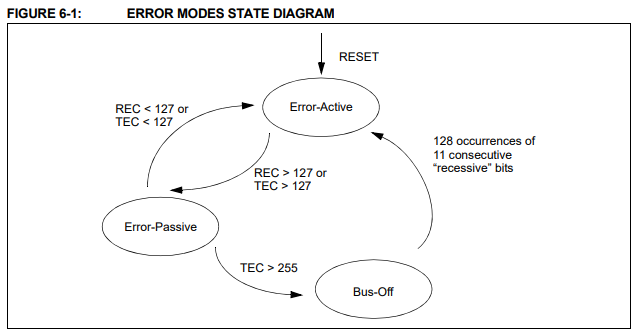
\includegraphics{../figures/Etat_CAN.png}
    \captionof{figure}{Diagramme d'état des modes d'erreurs (extrait de la datasheet du MCP2515)}
\end{minipage}

\medspace

Lorsque le bus est éteint, il est dans l'état STOPPED :
\vspace{-1.8\baselineskip} 
\begin{lstlisting}
    3: can0: <NOARP,UP,LOWER_UP,ECHO> mtu 16 qdisc pfifo_fast state UP mode DEFAULT group default qlen 10
    link/can  promiscuity 0 minmtu 0 maxmtu 0 
    can state STOPPED (berr-counter tx 0 rx 0) restart-ms 0 
	  bitrate 125000 sample-point 0.875 
	  tq 500 prop-seg 6 phase-seg1 7 phase-seg2 2 sjw 1
	  pcan_usb: tseg1 1..16 tseg2 1..8 sjw 1..4 brp 1..64 brp-inc 1
	  clock 8000000 numtxqueues 1 numrxqueues 1 gso_max_size 65536 gso_max_segs 65535 parentbus usb parentdev 2-2.1:1.0  
\end{lstlisting}


Lorsque le bus est fonctionnel, il est dans l'état ERROR-ACTIVE :
\vspace{-1.8\baselineskip} 
\begin{lstlisting}
    3: can0: <NOARP,UP,LOWER_UP,ECHO> mtu 16 qdisc pfifo_fast state UP mode DEFAULT group default qlen 10
    link/can  promiscuity 0 minmtu 0 maxmtu 0 
    can state ERROR-ACTIVE (berr-counter tx 0 rx 0) restart-ms 0 
	  bitrate 125000 sample-point 0.875 
	  tq 500 prop-seg 6 phase-seg1 7 phase-seg2 2 sjw 1
	  pcan_usb: tseg1 1..16 tseg2 1..8 sjw 1..4 brp 1..64 brp-inc 1
	  clock 8000000 numtxqueues 1 numrxqueues 1 gso_max_size 65536 gso_max_segs 65535 parentbus usb parentdev 2-2.1:1.0  
\end{lstlisting}

Lorsque le bus est en erreur, il est dans l'état ERROR-PASSIVE :
\vspace{-1.8\baselineskip} 
\begin{lstlisting}
    3: can0: <NOARP,UP,LOWER_UP,ECHO> mtu 16 qdisc pfifo_fast state UP mode DEFAULT group default qlen 10
    link/can  promiscuity 0 minmtu 0 maxmtu 0 
    can state ERROR-PASSIVE (berr-counter tx 0 rx 0) restart-ms 0 
	  bitrate 125000 sample-point 0.875 
	  tq 500 prop-seg 6 phase-seg1 7 phase-seg2 2 sjw 1
	  pcan_usb: tseg1 1..16 tseg2 1..8 sjw 1..4 brp 1..64 brp-inc 1
	  clock 8000000 numtxqueues 1 numrxqueues 1 gso_max_size 65536 gso_max_segs 65535 parentbus usb parentdev 2-2.1:1.0  
\end{lstlisting}
Dans cet état, il faut redémarrer le bus pour qu'il recommence à fonctionner. Pour cela, vous pouvez soit redémarrer la Raspberry Pi (dans le cas où le service est "enable" et se lance tout seul au boot de la Raspberry Pi), soit taper la commande : 
\vspace{-1.8\baselineskip} 
\begin{lstlisting}
    sudo systemctl restart can0.service
\end{lstlisting}

\subsubsection{Installation du Hotspot}
Afin de permettre au Smartphone de se connecter à la Raspberry Pi, il lui faut générer un Hotspot. 

Pour cela, vous pouvez suivre le tutoriel de ce site : \href{https://bentek.fr/creer-hotspot-wifi-sur-raspberry-pi/}{Créer un hotspot sur Raspberry Pi}.
\begin{enumerate}
    \item Installez RaspAP : \newline
    Création d'une sauvegarde du fichier de configuration WiFi :
\vspace{-1.8\baselineskip} 
\begin{lstlisting}
    sudo cp /etc/wpa_supplicant/wpa_supplicant.conf /etc/wpa_supplicant/wpa_supplicant.conf.sav
\end{lstlisting}
    Suppression du fichier de configuration WiFi pour retourner à une configuration vierge :
\vspace{-1.8\baselineskip} 
\begin{lstlisting}
    sudo cp /dev/null /etc/wpa_supplicant/wpa_supplicant.conf
\end{lstlisting}
    Téléchargement et installation de RaspAP :
\vspace{-1.8\baselineskip} 
\begin{lstlisting}
    wget -q https://git.io/voEUQ -O /tmp/raspap && bash /tmp/raspap
\end{lstlisting}
    \item Attendez la fin du téléchargement et redémarrez la Raspberry Pi.\newline
\end{enumerate}

Ce réseau est automatiquement déployé sur wlan0. Vous pouvez taper la commande suivante pour vérifier que le hotspot est en place : 
\vspace{-1.8\baselineskip} 
\begin{lstlisting}
    ip a
\end{lstlisting}
Vous devriez voir à minima :
\vspace{-1.8\baselineskip} 
\begin{lstlisting}
    wlan0: <BROADCAST,MULTICAST,UP,LOWER_UP> mtu 1500 qdisc pfifo_fast state UP group default qlen 1000
    link/ether b8:27:eb:7d:39:15 brd ff:ff:ff:ff:ff:ff
    inet 10.3.141.1/24 brd 10.3.141.255 scope global noprefixroute wlan0
       valid_lft forever preferred_lft forever
    inet6 fe80::bc4f:144b:a962:a45f/64 scope link 
       valid_lft forever preferred_lft forever
\end{lstlisting}

Vous pouvez connecter votre Smartphone ou votre PC au hotspot, le nom du réseau est "raspi-webgui". Le mot de passe est "ChangeMe".

L'interface d'adminitration de RaspAP est accessible en vous connectant au hotspot, tapez "10.3.141.1" dans un navigateur web. Par défaut, le nom d'utilisateur est "admin" et le mot de passe est "secret". Vous pouvez configurer le hotspot à votre convenance.

\subsection{Installation des outils pour compiler le programme {\nomLogiciel}}

\subsubsection{Installation du compilateur}

Afin de compiler le programme pour Raspberry Pi, il faut installer le compilateur ARM. Vous pouvez utiliser celui que vous souhaitez mais nous vous proposons ce tutoriel pour récupérer le compilateur utilisé lors du développement :
\begin{enumerate}
    \item Récupérer les outils de développement croisés : \newline
    Dans le dossier de votre choix, tapez la commande suivante :
\vspace{-1.8\baselineskip} 
\begin{lstlisting}
    git clone https://github.com/raspberrypi/tools.git
\end{lstlisting}
    \item Modifier le fichier "variable.mk" afin de renseigner le chemin absolu vers le compilateur (dossier où vous avez cloné le fichier précédemment) : modifez la variable "RASPBERRY\_TOOLS". \newline
\end{enumerate}

Si ce n'est pas déjà fait, pensez également à installer gcc sur votre machine, dans n'importe quel terminal, tapez : 
\vspace{-1.8\baselineskip} 
\begin{lstlisting}
    sudo apt install gcc
\end{lstlisting}

\subsubsection{Installation de CMocka}

Le programme {\nomLogiciel} est fourni avec des tests automatisés. Afin de compiler ces tests, vous avez besoin de la librairie CMocka. Les tests sont autant exécutables sur votre machine que sur cible. Si votre machine ne possède pas la même architecture que la Raspberry Pi, vous avez donc besoin de deux librairies différentes. Afin de faciliter l'utilisation de CMocka, nous vous proposons de compiler la librairie en statique. \newline

Le tutoriel est le même pour les deux architectures, la seule différence est que pour une compilation sur cible, vous devez compiler la librairie sur la cible, pour une compilation locale, vous devez compiler la librairie sur votre machine. \newline

Attention, afin de compiler la librairie, vous avez besoin de cmake et make, dans un terminal, tapez :
\vspace{-1.8\baselineskip} 
\begin{lstlisting}
    sudo apt install cmake
    sudo apt install make
\end{lstlisting}

\begin{enumerate}
    \item Téléchargez CMocka \href{https://cmocka.org/}{CMocka}, version 1.1.5.
    \item Consultez les fichier README et INSTALL pour plus d'informations sur l'installation de CMocka.
    \item Dans le fichier "DefineOptions.cmake" : 
\vspace{-1.8\baselineskip} 
\begin{lstlisting}
    option(WITH_STATIC_LIB "Build with a static library" ON)
\end{lstlisting}
    \item Créez un répertoire "build" dans le dossier de CMocka et allez dedans.
    \item Générez le Makefile avec cmake :
\vspace{-1.8\baselineskip} 
\begin{lstlisting}
    cmake -DCMAKE_INSTALL_PREFIX=<choisir un emplacement> ..
\end{lstlisting}
    \item Compilez et installez la librairie :
\vspace{-1.8\baselineskip} 
\begin{lstlisting}
    make
    make install
\end{lstlisting}
\end{enumerate}

Si vous avez compilez la librairie sur cible, vous pouvez récupérer les dossier "include" et "lib" dans le dossier d'installation que vous avez choisi et les installer sur votre machine. \newline
Vous pouvez utiliser la commande "scp" pour copier les dossiers de la cible vers votre machine :
Sur votre machine, tapez : 
\vspace{-1.8\baselineskip} 
\begin{lstlisting}
    scp -r <user>@<ip>:<chemin vers le dossier> <chemin vers le dossier de destination>
\end{lstlisting}

Après avoir récupéré les deux librairies, modifiez le fichier "variable.mk" afin de renseigner les chemins absolus vers les librairies : modifez la variable "CMOCKA" (Attention, elle est déclarée deux fois dans le fichier selon si la variable "TARGET" est égale à "raspberry" ou non).

\subsubsection{Compilation du programme {\nomLogiciel}}

Vous avez désormais tous les outils nécessaires pour compiler le programme {\nomLogiciel}. \newline

Comme expliqué précédemment, il est possible d'exécuter les tests automatisés sur cible et sur votre machine. \newline

Lorsque le programme est compilé sur cible, un script est appelé afin de transmettre l'exécutable à la Raspberry Pi. Pour que cela fonctionne, assurez-vous de pouvoir vous connecter à la Raspberry Pi en SSH. \newline

Vous pouvez modifier le fichier "transfert\_bin.sh" afin de renseigner le nom d'utilisateur et l'adresse IP de la Raspberry Pi. \newline
Dans le cas où votre Raspberry Pi aurait un port de connexion SSH différent de celui par défaut, pensez à modifier la commande "scp" du fichier afin de lui indiquer le port à utiliser : utilisez le paramètre "-P" suivi du numéro du port. \newline

Pour compiler : 
\begin{enumerate}
    \item Ouvrez un terminal dans le dossier "production". 
    \item Pour compiler sur cible, tapez :
\vspace{-1.8\baselineskip} 
\begin{lstlisting}
    make TARGET=raspberry
\end{lstlisting}
\newpage
    \item Pour compiler sur votre machine, tapez :
\vspace{-1.8\baselineskip} 
\begin{lstlisting}
    make 
\end{lstlisting}
\end{enumerate}

Une fois la compilation terminée, vous pouvez voir les exécutables "CANgateway.out" et "CANgateway\_test.out" dans le dossier "bin". \newline

Pour une compilation sur cible, les exécutables sont visibles dans le dossier /home/pi de la Raspberry Pi. \newline


% -------------------
% INSTALLATION ICSim
% -------------------
\section{Installation de ICSim}

Nous vous proposons un tutoriel d'installation du simulateur ICSim que nous avons utilisé pour développer notre système.

ICSim est un logiciel open source, pour l'installer, nous avons suivi les instructions du README.md du projet disponible sur GitHub : \href{https://github.com/zombieCraig/ICSim}{ICSim}. 

\medspace

Dans ce tutoriel, ICSim est lancé avec l'interface virtuelle vcan0. Il est cependant possible de l'utiliser avec une interface réelle. Pour cela, il faut remplacer vcan0 par can0 dans les commandes du README. 

\medspace

Attention, néanmoins, pour que l'interface CAN réelle fonctionne, vous devez avoir connecté votre PC à un device CAN. Dans le cas contraire, les commandes de configurations de l'interface CAN réelle ne fonctionneront pas. 

\medspace



% -------------------
% INSTALLATION ICSim
% -------------------
\section{Installation de JMeter}

Pour la réalisation des tests fonctionnels du serveur TCP implémenté dans le module Postman, nous avons utilisé JMeter.\\

JMeter est un outil open-source de test de performance et de charge développé par Apache. Il permet de mesurer et d'évaluer les performances d'une application web ou d'un serveur en simulant différents scénarios d'utilisation. JMeter offre une grande flexibilité pour la création de tests et fournit des statistiques détaillées sur les performances, la fiabilité et la capacité de l'application testée.\\

Tout d'abord, assurez-vous d'avoir une version récente de Java installée sur votre système, car JMeter est basé sur Java. Pour l'installer, rendez-vous sur le site officiel d'Oracle Java à l'adresse suivante : \href{https://www.oracle.com/java/technologies/javase-jdk11-downloads.html}{https://www.oracle.com/java/technologies/javase-jdk11-downloads.html}.
Dans notre cas nous avons installé le JDK (Java Development Kit) d'OpenJDK 11.\\

Pour installer JMeter il faut :
\begin{itemize}
    \item Allez sur le site officiel d'Apache JMeter à l'adresse suivante : \href{https://jmeter.apache.org/}{https://jmeter.apache.org/}.
    \item Dans la section "Downloads", cliquez sur le lien correspondant à la version la plus récente de JMeter. Vous serez redirigé vers la page de téléchargement.
    \item Sur la page de téléchargement, choisissez le fichier binaire qui correspond à votre système d'exploitation (Windows, Linux, Mac OS, etc.) et téléchargez-le sur votre ordinateur.
    \item Une fois le téléchargement terminé, décompressez le dossier dans le répertoire de votre choix.
    \item Accédez au répertoire extrait, allez dans le répertoire bin/ et lancez JMeter en exécutant le fichier "jmeter.bat" pour Windows ou "jmeter.sh" pour Linux/Mac OS.
    \item JMeter s'ouvrira avec une interface graphique. Vous êtes maintenant prêt à commencer à créer et exécuter des tests de performance.
\end{itemize}

\label{LastPage}
\end{document}
% ------------
% FIN DOCUMENT 
% ------------